\section{Algebra Boole'a}

Aksjomaty algebry Boole'a:
\begin{figure}[H]
    \centering
    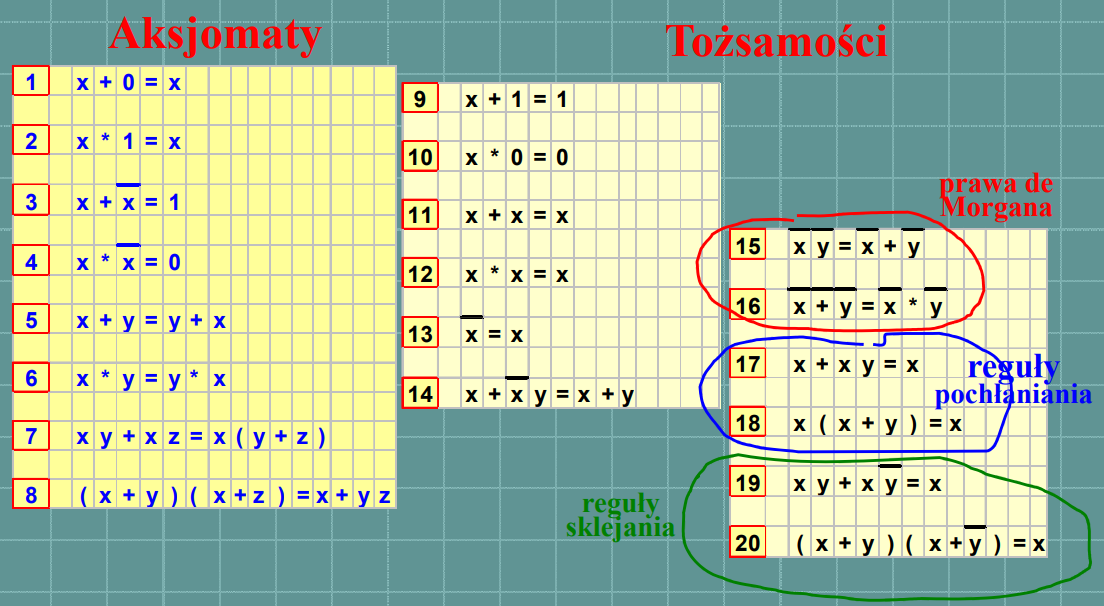
\includegraphics[width=1\textwidth]{img/aksjomaty.png}
    \caption{Aksjomaty algebry Boole'a}
\end{figure}

sprawdzenie tożsamości za pomocą tabeli prawdy:
\begin{enumerate}
    \item $(x+y)(x+z) = x + yz$
    \item $x + \overline{x}y = x + y$
\end{enumerate}

na podstawie aksjomatów i tożsamości można upraszczać wyrażenia.

Przykłady upraszczania wyrażeń:

\begin{enumerate}
    \item $\overline{x}\overline{y} + xy + \overline{x}y$
    \item $(x + y)(x + \overline{y})$
    \item $\overline{x} + xy + x\overline{z} + x\overline{y}\overline{z}$
    \item $\overline{(x+y)}(\overline{x} + \overline{y})$
    \item $xy + \overline{x}y\overline{z} + yz$
    \item $yz + xywz + \overline{y}z$ 
    \item $x\overline{y} + z + (\overline{x} + y)\overline{z}$
    \item $(x + \overline{y})(y + \overline{z})(z + \overline{x})(xyz + \bar{x}\bar{y}\bar{z})$
    \item $x\overline{y} + z(\overline{x} + y + w)$
    \item $(a + b)(\overline{\overline{ab} + \overline{a}c}) + \overline{c}$
    \item $(x + y)(x + y + z) + \bar{x}\bar{y} + \bar{x}\bar{z}$
    \item $xyz + xy\bar{z} + x\bar{y}z + x\bar{y}\bar{z} + \bar{x}z$
    \item $ab + \bar{c}\bar{d} + \bar{a}bc\bar{d} + a\bar{b}\bar{c}d$
\end{enumerate}

Odpowiedzi:
\begin{enumerate}
    \item $\overline{x} + y$
    \item $x$
    \item $\overline{x} + y + \overline{z}$
    \item $\overline{x}\overline{y}$
    \item $y$
    \item $z$
    \item $1$
    \item $xyz + \bar{x}\bar{y}\bar{z}$
    \item $z + x\overline{y}$
    \item $ab + \overline{c}$
    \item $1$
    \item $x + z$
    \item $(a + \bar{d})(b + \bar{c})$
\end{enumerate}